\documentclass[usenames,dvipsnames]{beamer}

\usetheme[
	progressbar=frametitle,
	titleformat section=smallcaps,
	subsectionpage=progressbar
]{metropolis}

\providecommand{\version}{local-dev}


% cSpell:disable
% chktex-file 15

% CLI arguments

\usepackage{ifthen}
\ifthenelse%
	{\equal{\generatenotes}{hide}}
	{\newcommand{\notesOption}{hide notes}}
	{
		\ifthenelse%
			{\equal{\generatenotes}{second}}
			{\newcommand{\notesOption}{show notes on second screen}}
			{\newcommand{\notesOption}{show only notes}}
	}%

% packages

\usepackage[
	orientation=landscape,
	size=custom,
	width=24,
	height=14,
	scale=0.6
]{beamerposter}

\usepackage{pgfpages}
\usepackage{booktabs}
\usepackage{bm}
\usepackage{mathtools}
\usepackage{listings}
\usepackage{fancybox}
\usepackage{bm}
\usepackage{multicol}
\usepackage{xpatch}
\usepackage{hyperref}
\usepackage{hyperxmp}
\usepackage{multirow}
\usepackage{xparse}
\usepackage{hyphenat}
\usepackage{xfrac}
\usepackage{caption}
\usepackage{enumitem}
\setitemize{label=	\usebeamerfont*{itemize item}
					\usebeamercolor[fg]{itemize item}
					\usebeamertemplate{itemize item}}

\usepackage{siunitx}
\sisetup{range-phrase=--}

\usepackage{natbib}
\bibliographystyle{natbib}

\usepackage{background}
\backgroundsetup{
	placement=center,
	scale=3,
	contents={\begin{minipage}{1.0\textwidth}\centering\wm\end{minipage}},
	opacity=0.02,
	color=gray,
	angle=0
}
\setbeamertemplate{background}{\BgMaterial}


% settings

\graphicspath{{./graphics/}}

\makeatletter
\defbeameroption{show only notes}[]%
{
	\beamer@notestrue%
	\beamer@notesnormalsfalse%
}
\makeatother

\setbeameroption{\notesOption}

\setsansfont{CMU Serif}
\setmonofont{CMU Typewriter Text}

\makeatletter
\let\@@magyar@captionfix\relax % chktex 21
\makeatother

\logo{
	
\includegraphics[
		width=2cm,
		keepaspectratio
	]{logo}\hspace{\dimexpr\paperwidth-2cm-10pt}\vspace{-30pt}
}

\titlegraphic{%
	\begin{picture}(0,0)
		\put(620,-180){\makebox(0,0)[rt]{
\includegraphics[width=5cm]{logo}}}
	\end{picture}
}

\makeatletter
	\def\beamer@framenotesbegin{% at beginning of slide
		\usebeamercolor[fg]{normal text}
			\gdef\beamer@noteitems{}%
			\gdef\beamer@notes{}%
	}
\makeatother

\definecolor{RoyalBlue}{RGB}{11,32,76}
\definecolor{DustyBlue}{RGB}{81,150,195}

\hypersetup{
	colorlinks=true,
	linkcolor=RoyalBlue,
	urlcolor=RoyalBlue,
	citecolor=DustyBlue,
	pdfpagemode=FullScreen,
	pdfdisplaydoctitle=true,
	pdfmenubar=false,
	pdfpagelayout=SinglePage
}

\captionsetup[figure]{labelformat=empty}

\makeatletter
	\setlength{\metropolis@progressinheadfoot@linewidth}{2pt}
\makeatother

\setbeamercolor{background canvas}{bg=white}
\setbeamercolor{normal text}{fg=RoyalBlue}
\setbeamercolor{alerted text}{fg=DustyBlue}
\setbeamercolor{example text}{fg=RoyalBlue}
{
	\usebeamercolor[fg]{alerted text}
	\usebeamercolor[fg]{example text}
	\usebeamercolor[fg]{normal text}
}

% definitions

\xpatchbibmacro{name:andothers}{%
	\bibstring{andothers}%
}{%
	\bibstring[\emph]{andothers}%
}{}{}

\makeatletter
	\newcommand{\manuallabel}[2]{\def\@currentlabel{#2}\label{#1}} % chktex 21
\makeatother

\newenvironment<>{fixblock}[1]{%
	\begin{block}{#1}
		\vspace{0pt}
		#2
}{
	\end{block}
}

\newenvironment{fixnote}{\startfixnote}{}
\def\startfixnote#1\end{\note{#1}\end} % chktex 9 chktex 14


\title{Dissertation Defense}

\subtitle{
	Secure and Efficient Query Processing in Outsourced Databases \\
	{\small Range Queries~\cite{ore-benchmark-17, epsolute}, Point Queries~\cite{epsolute}, \knn{} Queries}
}

\date{Built from \href{https://git.dbogatov.org/bu/defense/presentation/commit/\version}{\emph{\version}} on \today}

\author{Dmytro Bogatov \\ \email{dmytro@bu.edu}}

\institute{Boston University \\ Graduate School of Arts and Sciences \\ Department of Computer Science}

\def\wm{
\includegraphics[keepaspectratio, width=0.1\textwidth]{coat-of-arms-1}}


\begin{document}

	\nobibliography*

	\maketitle

	\setbeamercovered{transparent}

	\section{Introduction}

	\begin{frame}{Motivation}

		Organizations outsource vast amounts of data to the cloud.
		

		% \begin{fixblock}{Block title}

			% Block content with formula

			\[
				P(x) = \frac{1}{{\sigma \sqrt{ 2 \pi } }} e^{ - \frac{(x - \mu)^2}{2 \sigma^2} }
			\]

		% \end{fixblock}

		\begin{itemize}
			\item Some list
			\item Some list
		\end{itemize}

		\note{
			The note.

		}

	\end{frame}


	\section{A comparative evaluation of order-revealing encryption schemes and secure range-query protocols~\cite{ore-benchmark-17}}

	\begin{frame}[label={frame:ore}]

		\frametitle{Survey of OPE/ORE schemes~\cite{ore-benchmark-17}}

		\begin{columns}[T,onlytextwidth]
			\column{0.5\textwidth}

				\begin{block}{The problem}

					\begin{itemize}
						\item Model: \alert{snapshot}, query type: \alert{range}
						\item Performance / security tradeoff
						\item Heterogeneous security definitions and leakage profiles
						\item \textbf{Performance of the schemes not well-understood}
						\begin{itemize}
							\item Some were not even implemented
							\item Prototype implementation at best
							\item Not benchmarked against one another
							\item Use different primitive implementations
						\end{itemize}
					\end{itemize}

				\end{block}

			\column{0.5\textwidth}

				\onslide<2->{
					\begin{block}{Our solution}

						\begin{itemize}
							\item Analyzed security and leakages of the constructions under a common framework
							\item Analyzed theoretically performance of the constructions
							\item \textbf{Implemented and ran experiments}
							\begin{itemize}
								\item Implemented 5 OPE / ORE schemes and 5 range query protocols
								\item Used same language, framework and primitive implementations
								\item Benchmarked primitives execution times
								\item Counted primitives and I/O usage
								\item[]
									\hyperlink{frame:appendix:ore}{\beamerskipbutton{ORE table}}
									\hyperlink{frame:appendix:protocols}{\beamerskipbutton{Protocols table}}
									\hyperlink{frame:appendix:plot}{\beamerskipbutton{Plot}}
							\end{itemize}
						\end{itemize}

					\end{block}
				}

		\end{columns}

	\end{frame}

	\section{\epsolute{}: Efficiently Querying Databases While Providing Differential Privacy~\cite{epsolute}}

	\begin{frame}{Differential Privacy and Sanitization}

		\begin{definition}[\alert{Differential Privacy}, adapted from~\cite{our-data-ourselves, differential-privacy-original}]
			\justify%

			A randomized algorithm \algo{A} is $(\epsilon, \delta)$-differentially private if for all $\database_1 \sim \database_2 \in \searchKeyDomain^\dataSize$, and for all subsets $\mathcal{O}$ of the output space of \algo{A},
			\[
				\probability{ \algo{A}{ \database_1 } \in \mathcal{O} } \leq \exp(\epsilon) \cdot \probability{ \algo{A}{ \database_2 } \in \mathcal{O} } + \delta \; .
			\]
		\end{definition}

		\pause%

		\begin{theorem}[\alert{Laplace Perturbation Algorithm (LPA)}, adapted Theorem 1 from~\cite{differential-privacy-original}]
			\justify%

			An algorithm \algo{A} that adds independently generated noise from a \textbf{zero-mean Laplace distribution} with scale $\lambda = \frac{\textsf{sensitivity of query}}{\epsilon}$ to each coordinate of a query result, satisfies $\epsilon$-differential privacy.
		\end{theorem}

		\pause%

		\begin{definition}[\alert{Differentially Private Sanitizer}, informal]
			\justify%

			An $(\epsilon, \delta, \alpha, \beta)$-differentially private sanitizer is a pair of algorithms $(\algo{A}, \algo{B})$ such that:
			\begin{itemize}
				\item $A$ is $(\epsilon, \delta)$-differentially private, and
				\item on input a dataset, \algo{A} outputs a data structure \serverDS{} such that with probability $1 - \beta$ for all queries, $\algo{B}{ \serverDS, \query }$ is within $\alpha$ of a real query result.
			\end{itemize}
		\end{definition}

	\end{frame}

	\begin{frame}{Background: Access pattern and ORAM}

		\justifying%

		\textbf{Access pattern} is a sequence of memory accesses \oramProgram{}, where each access consists of the memory \emph{location} $o$, read \oramRead{} or write \oramWrite{} \emph{operation} and the \emph{data} $d$ to be written.

		Oblivious RAM (ORAM) is a mechanism that hides the accesses pattern.
		More formally, \oram{} is a protocol between the client \client{} (who accesses) and the server \server{} (who stores), with a guarantee that the view of the server is indistinguishable for any two sequences of the same lengths.

		\begin{columns}[T]
			\column{0.475\textwidth}

				\[
					\begin{split}
						\abs{\oramProgram_1}					& = \abs{\oramProgram_2}							\\
						\textsc{View}_\server (\oramProgram_1)	& \cindist \textsc{View}_\server (\oramProgram_2)
					\end{split}
				\]

			\column{0.475\textwidth}

				\procedure[linenumbering]{\oram{} protocol}{
					\textbf{Client \client}											\>														\> \textbf{Server \server}	\\
					%
					\oramProgram{} = \left. (\oramRead, i, \bot) \right|_{i = 1}^5	\> 														\>							\\
					%
					\text{(client state)}											\> \sendmessageboth*[6em]{\algo{ORAM}{\oramProgram}}	\> \text{(server state)}	\\
					%
					\{ d_1, d_2, d_3, d_4, d_5 \}									\>														\>
				}

		\end{columns}

		\vspace*{1ex}

		For example: Square Root ORAM~\cite{oram-theory}, Hierarchical ORAM~\cite{oram-original}, Binary-Tree ORAM~\cite{binary-tree-oram}, Interleave Buffer Shuffle Square Root ORAM~\cite{shortest-path-oram}, TP-ORAM~\cite{tp-oram}, \textbf{Path-ORAM}~\cite{path-oram} and TaORAM~\cite{taostore}.
		\alert{ORAM incurs at least logarithmic overhead in the number of stored records.~\cite{oram-original}}

	\end{frame}

	\begin{frame}{Differentially Private Outsourced Database System}

		Model: \alert{persistent}, query type: \alert{point} and \alert{range}

		\begin{definition}[\alert{Computationally Differentially Private Outsourced Database System (CDP-ODB)}]
			\justify%

			We say that an outsourced database system \protocol{} is $(\epsilon, \delta)$-computationally differentially private (a.k.a.~CDP-ODB) if for every polynomial time distinguishing adversary \adversary{}, for every neighboring databases $\database \sim \database^\prime$, and for every query sequence $\fromNtoM{\query}{1}{m} \in \querySet^m$ where $m = \mathsf{poly}(\lambda)$,

			\begin{multline*}
				\probability{\adversary \left( 1^\lambda, \view{\protocol, \server}{\database, \fromNtoM{\query}{1}{m}} \right) = 1 } \leq \\
				\exp{\epsilon} \cdot \probability{\adversary \left( 1^\lambda, \view{\protocol ,\server}{\database^\prime, \fromNtoM{\query}{1}{m}} \right) = 1} + \delta + \negl \; ,
			\end{multline*}
			the probability is over the randomness of the distinguishing adversary \adversary{} and the protocol \protocol{}.
		\end{definition}

		\pause%

		Note:
		\begin{itemize}
			\item Entire view of the adversary is DP-protected
			\item Implies protection against communication volume and access pattern leakages
			\item Query sequence $\fromNtoM{\query}{1}{m} \in \querySet^m$ is fixed
			\item $\negl$ accounts for the computational (as opposed to theoretical) DP definition
		\end{itemize}

	\end{frame}

	\begin{frame}{On impossibility of adaptive queries}

		\begin{block}{Example}
			\justify%

			\begin{itemize}
				\item Suppose neighboring medical databases differ in one record with a rare diagnosis ``Alzheimer's disease''
				\item A medical professional queries the database
				\begin{itemize}
					\item
						for that diagnosis first (point query) \\
						\texttt{SELECT name FROM patients WHERE condition = 'ALZ'} % chktex 32

					\item
						if there is a record, she queries the senior patients next (range query) \\
						\texttt{SELECT name FROM patients WHERE age >= 65}

					\item
						otherwise she queries the general population,resulting in more records \\
						\texttt{SELECT name FROM patients}
				\end{itemize}
				\item Efficient system cannot return nearly the same number of records in both cases, thus, the adversary can distinguish
			\end{itemize}

		\end{block}

	\end{frame}

	\begin{frame}{Single-Threaded \epsolute{}}

		\centering
		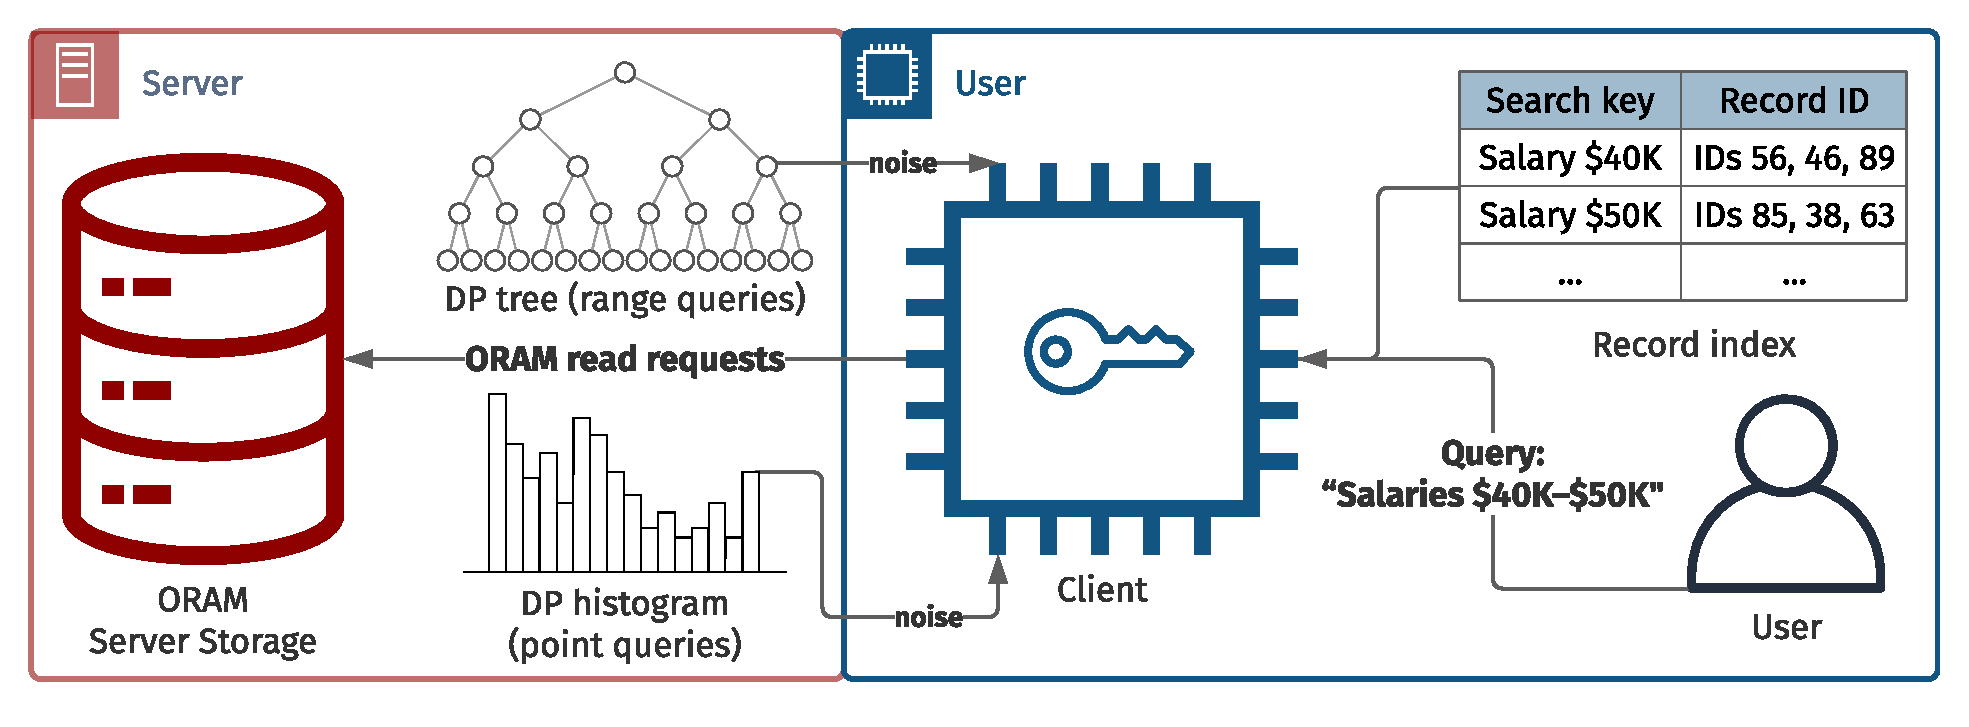
\includegraphics[width=\textwidth]{dp-oram}

	\end{frame}

	\begin{frame}{Parallel \epsolute{}: the choice of separate vs shared \serverDS{}}

		\onslide<1->{
			\begin{itemize}
				\item Split \user{} and \server{} state into \oramsNumber{} ORAMs, run as separate machines
				\item Partition records randomly (by ID) into \oramsNumber{} partitions, generate \oramsNumber{} inverted indexes
				\item Choose a strategy on shared vs split \serverDS{}
			\end{itemize}
		}

		\begin{columns}[T]
			\begin{column}{0.5\textwidth}

				\onslide<2->{
					\begin{block}{No-$\gamma$ method: \serverDS{} per ORAM}

						\begin{itemize}[leftmargin=*]
							\item Composition of disjoint datasets: take max $\epsilon$
							\item Each ORAM replies with $(1 + \gamma) \frac{k_0}{\oramsNumber{}}$ records, where $k_0$ is a required number of records
							\item To bound probability to $\beta$, use $\gamma = \sqrt{ \frac{-3 \oramsNumber \log \beta}{ k_0 } }$
						\end{itemize}

					\end{block}
				}

			\end{column}

			\begin{column}{0.5\textwidth}

				\onslide<3->{
					\begin{block}{$\gamma$-method: shared \serverDS{}}

						\begin{itemize}[leftmargin=*]
							\item Same number of records per ORAM
							\item
								Use $\gamma$ as in no-$\gamma$ method, except
								\begin{itemize}
									\item $k_0 \gets k_0 + \frac{\log \domainSize}{\epsilon}$ for point queries
									\item $k_0 \gets k_0 + \frac{\log^{1.5} \domainSize}{\epsilon}$ for range queries
								\end{itemize}

						\end{itemize}

					\end{block}
				}

			\end{column}

		\end{columns}

	\end{frame}

	\begin{frame}{Parallel \epsolute{} diagram (with improvements)}

		\centering
		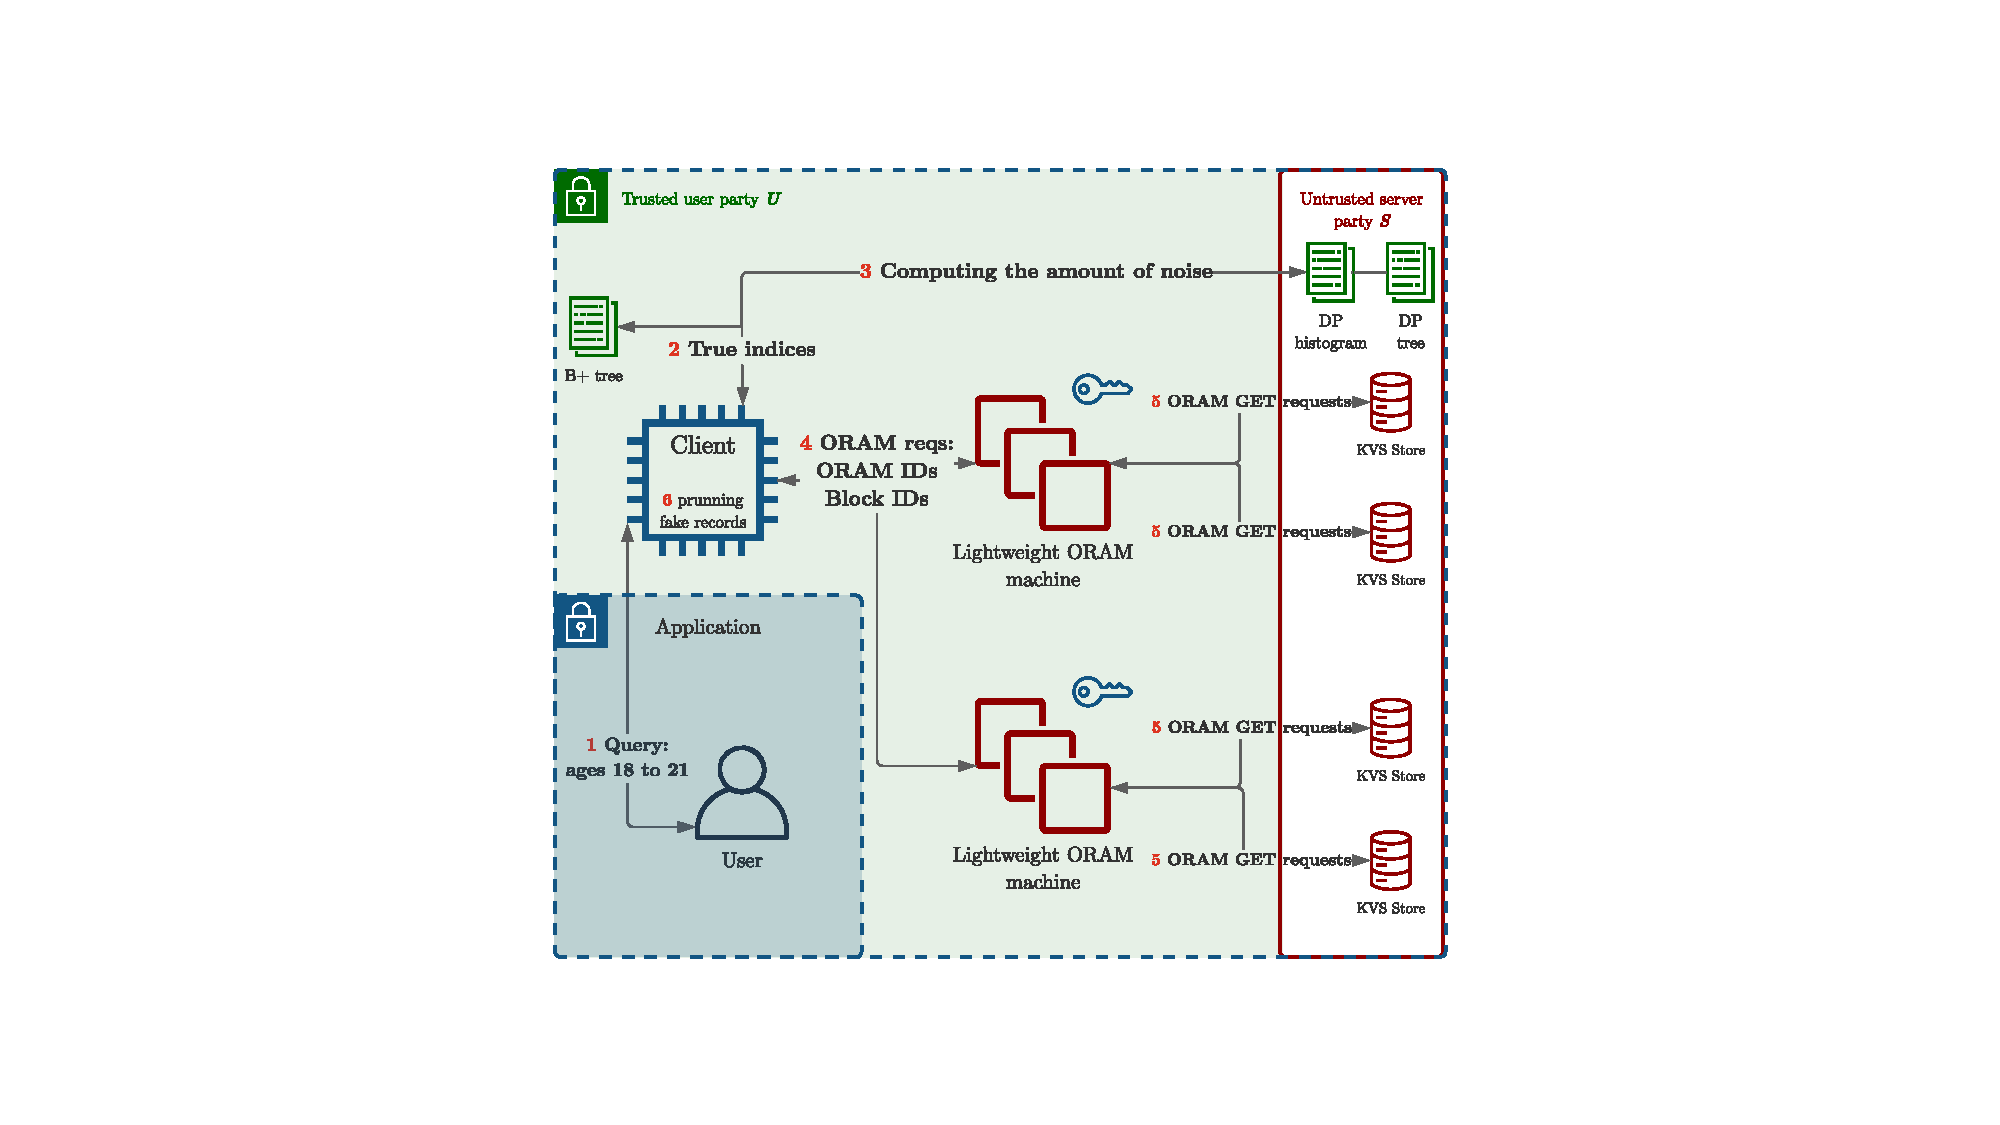
\includegraphics[scale=0.44]{three-layers}

	\end{frame}

	\begin{frame}{Experiments: against other mechanisms}

		\begin{figure}[h]
			\centering
			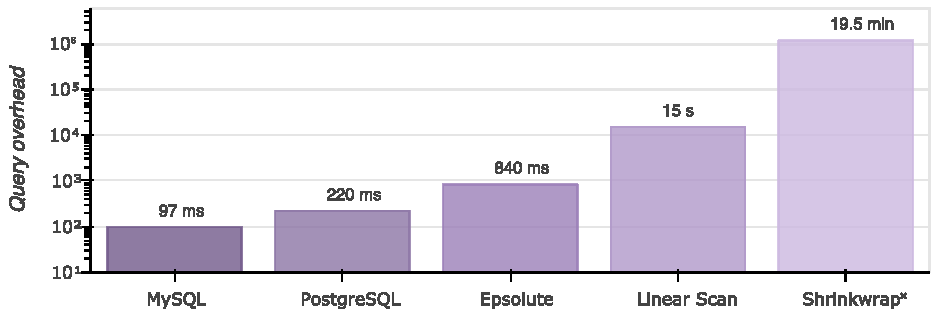
\includegraphics[width=\textwidth]{mechanism}
			\caption{
				\centering
				Different range-query mechanisms (log scale).
				Default setting: $10^6$ \SI{4}{\kibi\byte} uniformly-sampled records with the range $10^4$.
			}%
		\end{figure}

	\end{frame}

	\begin{frame}{Experiments: scalability}

		\begin{figure}[h]
			\centering
			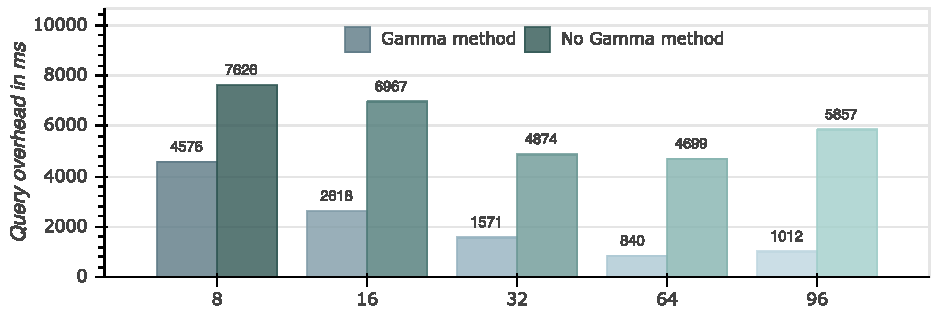
\includegraphics[width=\columnwidth]{scalability}
			\caption{Scalability measurements for \protocolGamma{} and \protocolNoGamma{}}%
		\end{figure}

	\end{frame}

	\section{Work-in-progress: \\ private \knn{} queries}

	\begin{frame}[label={frame:knn}]

		\frametitle{General idea}

		\begin{itemize}
			\item<1->
				Model: \alert{snapshot}, query type: \alert{\knn{}} in arbitrary dimensions

			\item<2->
				Input: vector of real numbers, query: return $k$ ``closest'' inputs to given vector \\
				\begin{small}
					Distance can be $\text{L}_\text{p}$ (usually, Euclidean, $p = 2$) or inner (dot) product
				\end{small}

			\item<3->
				Applications range from similarity search to geographical search \\
				\begin{small}
					Document is a vector of words/features/topics, query is to find $k$ most similar documents \\
					Object on a map is a 2D vector, query is to find $k$ nearest locations
				\end{small}

			\item<4->
				\emph{Approximate distance-comparison preserving encryption (DCPE) scheme} on input and queries
				\[
					\forall x, y, x \in \mathbb{X} : \algo{Dist}{x, y} < \algo{Dist}{x, z} - \beta \implies \algo{Dist}{f(x), f(y)} < \algo{Dist}{f(x), f(z)}
				\]

			\item<5->
				Prove theoretically and observe empirically how accuracy and efficiency of attacks drop with higher security \\
				\begin{small}
					\hyperlink{frame:appendix:dcpe}{\beamerskipbutton{DCPE}}
					\hyperlink{frame:appendix:trec-faiss}{\beamerskipbutton{TREC and FAISS}}
					\hyperlink{frame:appendix:knn-plot}{\beamerskipbutton{Intermediate results plot}}
				\end{small}

		\end{itemize}

	\end{frame}

	\section{Work-in-progress: \\ oblivious \texttt{JOIN}s}

	\begin{frame}[label={frame:oblivious-joins}]

		\frametitle{General idea}

		\begin{itemize}
			\item<1->
				Model: \alert{persistent}, query type: \alert{inner \texttt{JOIN}}

			\item<2->
				Input: two tables $T_1$ and $T_2$, query: return a cross product of $T_1$ and $T_2$ where $T_1.k = T_2.k$ \\
				\begin{small}
					We may also consider \texttt{SELECT JOIN}: \texttt{WHERE $T_1$.k = $T_2$.k AND $T_1$.a = 10}
				\end{small}

			\item<3->
				\alert{Challenge}: produce \texttt{JOIN} result hiding both access pattern and result size

			\item<4->
				\alert{Proposed solution}:
				\begin{itemize}
					\item use enclave (SGX) and oblivious primitives (sort, compaction)
					\item construct index over join keys, add DP noise to it
					\item partition the data by keys to fit a partition in the enclave
					\item consolidate sparse keys as an optimization
					\item do inner join within partition
					\item[] \hyperlink{frame:appendix:joins-detailed}{\beamerskipbutton{Detailed Algorithm}}
				\end{itemize}

		\end{itemize}

	\end{frame}



	\maketitle

	\backupbegin%

	\ifthenelse%
		{\equal{\generatenotes}{only}}
		{\nocite{*}}
		{}

	\begin{frame}[allowframebreaks]{References}

		\bibliography{bibfile}

		\note{The references}

	\end{frame}

	\appendix

	\section{Appendix}

	\begin{frame}[label={frame:appendix:ore}]

		\frametitle{OPE / ORE schemes}

		\begin{adjustbox}{width=\linewidth}
			\begin{tabular}{ l c c c c c }

				\toprule

				\multirow{2}{*}{Scheme}						& \multicolumn{2}{c}{\onslide<1->{Primitive usage}}																						& \onslide<1->{Ciphertext size,}																& \onslide<1->{Leakage}																\onslide<1->{\\ \cline{2-3}}
				\rule{0pt}{10pt}							& \onslide<1->{Encryption}													& \onslide<1->{Comparison}									& \onslide<1->{or state size}																	& \onslide<1->{(in addition to inherent total order)}								\\

				\toprule

				BCLO \cite{crypt-db-ope}					& \onslide<1->{$\bm{n}$ \textbf{HG}}										& \onslide<1->{none}										& \onslide<1->{$2n$}																			& \onslide<1->{\textbf{$\approx$ Top half of the bits}}								\\

				\midrule

				CLWW \cite{practical-ore}					& \onslide<1->{$n$ PRF} 													& \onslide<1->{none}										& \onslide<1->{$2n$}																			& \onslide<1->{\textbf{Most-significant differing bit}}								\\

				\midrule

				\multirow{3}{*}{Lewi-Wu \cite{lewi-ore}}	& \onslide<1->{\boldmath{} $\nicefrac{2n}{d}$ \unboldmath{} \textbf{PRP}}	& \onslide<1->{\multirow{3}{*}{$\frac{n}{2d}$ Hash}}		& \onslide<1->{\multirow{3}{*}{$\frac{n}{d} \left(\lambda + n + 2^{d + 1} \right) + \lambda$}}	& \onslide<1->{\multirow{3}{*}{Most-significant differing block}}					\\
															& \onslide<1->{$2 \frac{n}{d} \left( 2^d + 1 \right)$ PRF}					&															&																								&																					\\
															& \onslide<1->{$\frac{n}{d} 2^d$ Hash}										&															&																								&																					\\

				\midrule

				\multirow{3}{*}{CLOZ \cite{adam-ore-v2}}	& \onslide<1->{$n$ PRF}														& \onslide<1->{\multirow{3}{*}{$\bm{n^2}$ \textbf{PPH}}}	& \onslide<1->{\multirow{3}{*}{$n \cdot h$}}													& \onslide<1->{\multirow{3}{*}{Equality pattern of most-significant differing bit}}	\\
															& \onslide<1->{$n$ PPH}														&															&																								&																					\\
															& \onslide<1->{1 PRP}														&															&																								&																					\\

				\midrule

				FH-OPE \cite{fh-ope}						& \onslide<1->{1 Traversal}													& \onslide<1->{3 Traversals}								& \onslide<1->{$\bm{3 \cdot n \cdot N}$}														& \onslide<1->{Insertion order}														\\

				\bottomrule

			\end{tabular}
		\end{adjustbox}

		\hyperlink{frame:ore}{\beamerreturnbutton{Back to ORE}}

	\end{frame}

	\begin{frame}[label={frame:appendix:protocols}]

		\frametitle{Range query protocols}

		\begin{adjustbox}{width=\linewidth}
			\begin{tabular}{ l c c c c c c }

				\toprule

				\multirow{2}{*}{Protocol}						& \multicolumn{2}{c}{\onslide<1->{{\IO} requests}}																																& \multirow{2}{*}{\onslide<1->{Leakage}}	& \multicolumn{2}{c}{\onslide<1->{Communication (result excluded)}}																&	\onslide<1->{\\ \cline{2-3} \cline{5-6}}
				\rule{0pt}{10pt}								& \onslide<1->{Construction}									& \onslide<1->{Query}																							&											& \onslide<1->{Construction}									& \onslide<1->{Query} 											&	\\

				\toprule

				{\BPlus} tree with ORE							& \onslide<1->{$\log_B \frac{N}{B}$}							& \onslide<1->{$\log_B \frac{N}{B} + \frac{r}{B}$}																& \onslide<1->{\textbf{Same as ORE}}		& \onslide<1->{$1$}												& \onslide<1->{$1$}												&	\\
				\midrule

				Kerschbaum \cite{florian-protocol}				& \onslide<1->{$\bm{\frac{N}{B}}$}								& \onslide<1->{$\log_2 \frac{N}{B} + \frac{r}{B}$}																& \onslide<1->{\textbf{Total order}}		& \onslide<1->{$\log_2 N$}										& \onslide<1->{$\log_2 N$}										&	\\

				\midrule

				POPE \cite{pope} warm							& \multirow{2}{*}{\onslide<1->{$1$}}							& \onslide<1->{$\log_L \frac{N}{B} + \frac{r}{B}$}																& \onslide<1->{\textbf{Partial order}}		& \multirow{2}{*}{\onslide<1->{$1$}}							& \onslide<1->{$\log_L N$}										&	\\

				POPE \cite{pope} cold							& 																& \onslide<1->{$\bm{{\nicefrac{N}{B}}}$}																		& \onslide<1->{Fully hiding}				& 																& \onslide<1->{$\bm{N}$}										&	\\

				\midrule

				Logarithmic-BRC \cite{practical-range-search}	& \onslide<1->{\textbf{---}}									& \onslide<1->{$\bm{r}$}																						& \onslide<1->{Same as SSE}					& \onslide<1->{\textbf{---}}									& \onslide<1->{$\log_2 N$}										&	\\

				\midrule

				\multirow{2}{*}{ORAM}							& \multirow{2}{*}{\onslide<1->{$\bm{{ \log^2 \frac{N}{B} }}$}}	& \multirow{2}{*}{\onslide<1->{$\bm{{ \log_2 \frac{N}{B} \left( \log_B \frac{N}{B} + \frac{r}{B} \right) }}$}}	& \onslide<1->{Fully hiding}				& \multirow{2}{*}{\onslide<1->{$\bm{{ \log^2 \frac{N}{B} }}$}}	& \multirow{2}{*}{\onslide<1->{$\bm{{ \log^2 \frac{N}{B} }}$}}	&	\\
																&																&																												& \onslide<1->{(access pattern)}			&																&																&	\\

				\bottomrule

			\end{tabular}
		\end{adjustbox}

		\hyperlink{frame:ore}{\beamerreturnbutton{Back to ORE}}

	\end{frame}

	\begin{frame}[label={frame:appendix:plot}]

		\frametitle{One of the experimental results}

		\begin{figure}[h]
			\centering
			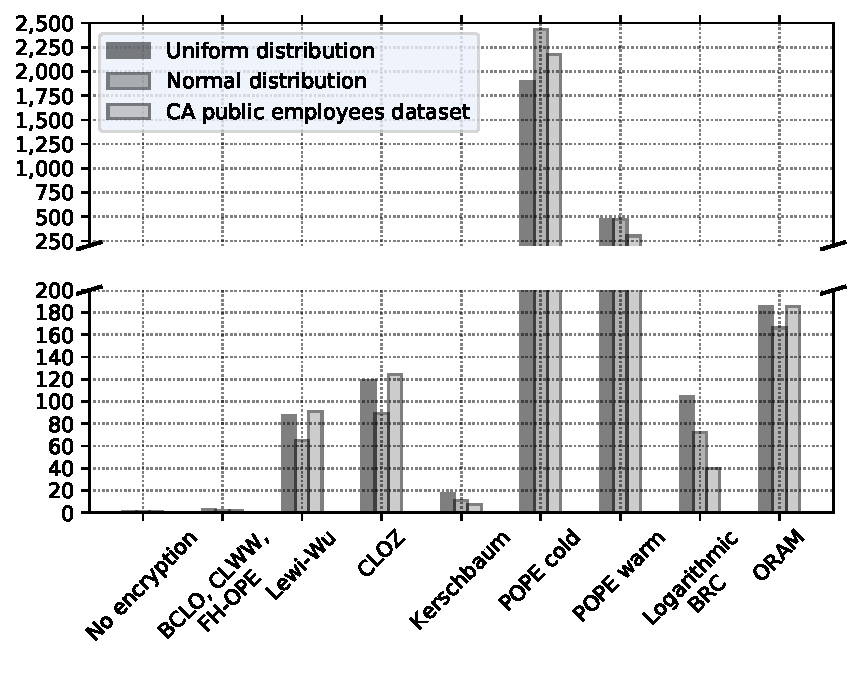
\includegraphics[width=0.6\textwidth]{protocol-charts-qios}
			\caption{
				Query stage number of I/O requests \\
				\hyperlink{frame:ore}{\beamerreturnbutton{Back to ORE}}
			}
		\end{figure}

	\end{frame}

	\begin{frame}[label={frame:appendix:oram}]

		\frametitle{Access pattern and ORAM}

		\justifying%

		\textbf{Access pattern} is a sequence of memory accesses \oramProgram{}, where each access consists of the memory \emph{location} $o$, read \oramRead{} or write \oramWrite{} \emph{operation} and the \emph{data} $d$ to be written.

		Oblivious RAM (ORAM) is a mechanism that hides the accesses pattern.
		More formally, \oram{} is a protocol between the client \client{} (who accesses) and the server \server{} (who stores), with a guarantee that the view of the server is indistinguishable for any two sequences of the same lengths.

		\begin{columns}[T]
			\column{0.475\textwidth}

				\[
					\begin{split}
						\abs{\oramProgram_1}					& = \abs{\oramProgram_2}							\\
						\textsc{View}_\server (\oramProgram_1)	& \cindist \textsc{View}_\server (\oramProgram_2)
					\end{split}
				\]

			\column{0.475\textwidth}

				\procedure[linenumbering]{\oram{} protocol}{
					\textbf{Client \client}											\>														\> \textbf{Server \server}	\\
					%
					\oramProgram{} = \left. (\oramRead, i, \bot) \right|_{i = 1}^5	\> 														\>							\\
					%
					\text{(client state)}											\> \sendmessageboth*[6em]{\algo{ORAM}{\oramProgram}}	\> \text{(server state)}	\\
					%
					\{ d_1, d_2, d_3, d_4, d_5 \}									\>														\>
				}

		\end{columns}

		\vspace*{1ex}

		Square Root ORAM \cite{oram-theory}, Hierarchical ORAM \cite{oram-original}, Binary-Tree ORAM \cite{binary-tree-oram}, Interleave Buffer Shuffle Square Root ORAM \cite{shortest-path-oram}, TP-ORAM \cite{tp-oram}, \textbf{Path-ORAM} \cite{path-oram} and TaORAM \cite{taostore}.
		\alert{ORAM incurs at least logarithmic overhead in the number of stored records. \cite{oram-original}}

		\begin{flushright}
			\hyperlink{frame:epsolute-motivation}{\beamerreturnbutton{Back to \epsolute{}}}
		\end{flushright}

	\end{frame}

	% chktex-file 1
	% chktex-file 8

	\begin{frame}[fragile,label={frame:appendix:dcpe}]

		\frametitle{Distance Comparison Preserving Encryption algorithms \cite{dcpe}}

		\justifying%

		\newlength{\algSeparationLength}
		\setlength{\algSeparationLength}{5.25em}

		\begin{algorithm}[H]

			\begin{pchstack}

				\procedure[linenumbering]{\algo{KeyGen}{\secparam, \mathbb{S}}}{
					s \sample \mathbb{S}		\\
					\key \sample \bin^\secpar	\\
					\pcreturn (s, \key)
				}

				\hspace*{\algSeparationLength}

				\procedure[linenumbering]{\algo{Enc}{ (s, \key), \vec{m} }}{
					n \sample \bin^\secpar														\\
					\mathsf{coins}_n || \mathsf{coins}_u \gets \algo{prf}{\key, n}	\\
					\vec{n} \sample \algo{Normal}{0, I_d; \mathsf{coins}_n}						\\
					u \sample \algo{Uniform}{0, 1; \mathsf{coins}_u}							\\
					x \gets \frac{s \beta}{4} \cdot \sqrt[d]{u}									\\
					\vec{\delta} \gets \frac{\vec{n}}{\|\vec{n}\|} \cdot x						\\
					\vec{c} \gets s \cdot \vec{m} + \vec{\delta}								\\
					\pcreturn \vec{c}
				}

				\hspace*{\algSeparationLength}

				\procedure[linenumbering]{\algo{Dec}{ (s, \key), (\vec{c}, n) }}{
					\mathsf{coins}_n || \mathsf{coins}_u \gets \algo{prf}{\key, n}	\\
					\vec{n} \sample \algo{Normal}{0, I_d; \mathsf{coins}_n}						\\
					u \sample \algo{Uniform}{0, 1; \mathsf{coins}_u}							\\
					x \gets \frac{s \beta}{4} \cdot \sqrt[d]{u}									\\
					\vec{\delta} \gets \frac{\vec{n}}{\|\vec{n}\|} \cdot x						\\
					\vec{m} \gets \frac{\vec{c} - \vec{\delta}}{s}								\\
					\pcreturn \vec{m}
				}

			\end{pchstack}

			\caption{Distance Comparison Preserving Encryption, adapted from \cite[Algorithm 2]{dcpe}}

		\end{algorithm}

		\begin{flushright}
			\hyperlink{frame:dcpe}{\beamerreturnbutton{Back to Private \knn{}}}
		\end{flushright}

	\end{frame}


	\backupend%

\end{document}
